\section{Implementation}

For long code snippets, we recommend to put them into the appendix of the
report. However, do not forget to reference them in the text. Small code
snippets can also be put directly alongside the respective paragraphs.

\subsection{Resources}

This section is supposed to enumerate (at least) \emph{four} helpful resources
that you conducted during implementation (e.g., the official documentation of
the chosen system). Briefly discuss in which respect the respective resources
were useful (1 paragraph each).

Although not mandatory, we would like to encourage you to list \emph{all}
resources that were useful to you (even without description).

\begin{packed_enum}
   \item \ldots
   \item \ldots
   \item \ldots
   \item \ldots
   \item Additional resource \ldots
\end{packed_enum}

\subsection{Setup}

Describe the machine setup thoroughly. This section serves as documentation of
your setup such that someone else could read through it and deploy your
application on a different machine after configuring this machine accordingly.
This includes (but is not limited to) the operating system of your (virtual)
machine, third-party tools/libraries, or modifications to configuration files.
Also explain why the respective tools/modifications were required/necessary in
order to get your application running (or maybe you just used/modified them for
convenience, which would also be okay).

\subsubsection{Server-Setup}
We used an instance of Amazon's EC2 Server\footnote{https://aws.amazon.com/de/ec2/}. The server's free trial period lasts for one year, so no fees were charged. We deployed an Ubuntu 16.04 LTS\footnote{http://releases.ubuntu.com/16.04/} instance to the server. When the creation is finished, you receive a SSH-Key for the default user (ubuntu). You can use this key to log into the server.

\paragraph{General Setup}
With the following commands for each team member (kard, sprs, schf) an user is created, sudo access granted and a SSH key pair generated. The following process can be repeated for any user. 
\\\\
Creates an user, \textit{-m} creates a home directory for that user too.
\begin{lstlisting}
sudo useradd -m kard
\end{lstlisting}

Grants root access to the given user.
\begin{lstlisting}
sudo usermod -a -G sudo kard
\end{lstlisting}

Sets a password for the given user, this could be any string generated with random.org, \textit{-e} states that the user has to change the password during his or her next login.
\begin{lstlisting}
sudo passwd kard -e
\end{lstlisting}

The following statement generates a key pair which will later be used to login and needs to be executed on the client as the generated private key should not pass the network (also make sure that ssh-keygen is installed).
\begin{lstlisting}
ssh-keygen nsdb-aws-kard
\end{lstlisting}

Next we will create an \textit{.ssh} directory in the user's home directory and create a file with the authorized keys in it, which will now be empty.
\begin{lstlisting}
mkdir .ssh
touch .ssh/authorized_keys
\end{lstlisting}

The public key can now be transferred to the server (e.g. the /tmp/ directory is suitable). Then the content of the key will be appended to the \textit{authorized\_keys} file.
\begin{lstlisting}
cat /tmp/nsdb-aws-kard.pub >> /home/kard/.ssh/authorized_keys
\end{lstlisting}

After that the permissions of the directory and the key file need to be adapted in order to be read by the ssh-server.
\begin{lstlisting}
sudo chown -R kard:kard .ssh
sudo chmod 700 .ssh
sudo chmod 644 .ssh/authorized_keys
\end{lstlisting}

The user's private key can now be given to the user (make sure that the key is encrypted and the password is transferred on another medium). After that the user is able to login with the key. As we don't need the \textit{ubuntu} user anymore, we can delete him with his home directory.
\begin{lstlisting}
sudo deluser ubuntu --remove-home 
\end{lstlisting}

\paragraph{Security Settings}
To eliminate the risk of Brute-Force attacks, remote password login is prohibited. This can be done by adding the following line to the SSH config file (/etc/ssh/sshd\_config).
\begin{lstlisting}
PasswordAuthentication no
\end{lstlisting}

Also remote root login is prohibited by changing the following line
\begin{lstlisting}
PermitRootLogin prohibit-password
\end{lstlisting}
to
\begin{lstlisting}
PermitRootLogin no
\end{lstlisting}

We don't need any firewall on the server, as we can configure a firewall trough the cloud dashboard. We only permit traffic on port 22 (SSH), port 80 (HTTP) and port 443 (HTTPS).
\begin{figure}[H]
	\centering
	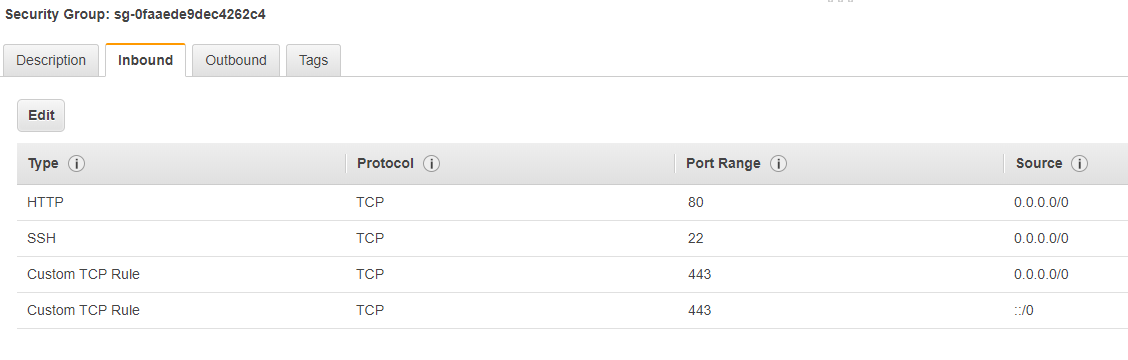
\includegraphics[width=\textwidth]{img/Security-Group}
	\caption{Firewall configuration for the instance}
	\label{fig:SecGroup}
\end{figure}

\subsection{Datasets}

If you use any additional or different datasets than specified in the previous
section/checkpoint, name them and discuss their characteristics (as required in
the previous section/checkpoint) (min. 1 paragraph per dataset).

If you generated your own synthetic datasets and made changes to the generation
process described in the previous section/checkpoint, discuss and justify these
changes here (min. 1 paragraph per dataset).

\subsubsection{Generation}

If you generated your own synthetic datasets, explain in detail how your
datasets are generated (including code snippets). This includes (but is not
limited to) the programming language/tools and how you ensure that your datasets
satisfy the desired characteristics.

\subsubsection{Import}

Discuss the import process here (including code snippets). Did you apply any
transformations before the data is stored in the underlying database system?
Which information is (not) stored? How is the information represented in the
underlying data model of your system?

If your datasets are of static nature, how long did it take you to import the
datasets? Did you put some effort into optimizing the import process? If so,
reason about the necessity (for example, because of very long runtimes without
optimizations) and briefly describe why the optimizations did (not) improve your
import process (1 paragraph each).

\subsection{Implementation}

Describe the actual implementation of your application. This subsection is
supposed to summarize all important parts/modules of your implementation
(including code snippets). For example, if you use other frameworks/libraries,
describe how they interact with the remaining parts of your application.

This section (including its subsection) is supposed to constitue the majority
of the report which is also reflected in the gradine scheme. Hence, this part of
the report should at least be 2-3 pages in total (text \emph{and} figures).

\subsubsection{Key System Features}

Discuss at least two key features of your underlying (database) system that you
used to implement (or optimize) your application (min. 1 paragraph each). For
a bonus point, discuss two other features you found useful in your application
context.

This includes (but is not limited to) indexes, views, replication, sharding,
transactions, specialized algorithms or data structures, aggregations, \ldots

\subsection{Problems Encountered}

\emph{Optional}. If any, summarize problems your encountered while implementing
your application. Briefly describe how you resolved the respective problems.
Moreover, if you had to make design decisions, discuss and justify them here.

\subsection{Alternative Implementation}

\emph{Optional}. Describe an implementation of your application that is based on
a different (database/processing) system (1-2 paragraphs). Briefly specify the
key parts of this alternative implementation (1 paragraph each) and discuss the
main differences to your original implementation (for example, limitations,
advantages/disadvantages, any other interesting aspect with respect to
performance, scalability, flexbility, \ldots) (1 paragraph each).
